\graphicspath{./Images}

\section{Honeycomb mechanics}
In order to develop a material model which accurately describes the mechanical behaviour of the aluminium honeycomb structures, it is key to identify the dominant failure mechanisms and understand the underlying physical phenomena. In this section, we will first focus on the relation between the geometrical structure of the material and the macroscopic mechanical behavior. Next, the currently existing techniques for modeling the honeycomb structures are discussed.
\subsection{Material characteristics}
The non-linear anisotropic behavior is for a large extend caused by the geometrical structure of the honeycomb material. Therefore, we first look at a top-view of the material geometry which is shown in Figure \ref{Ch2_topview}. 
\begin{figure}[H]
    \centering
    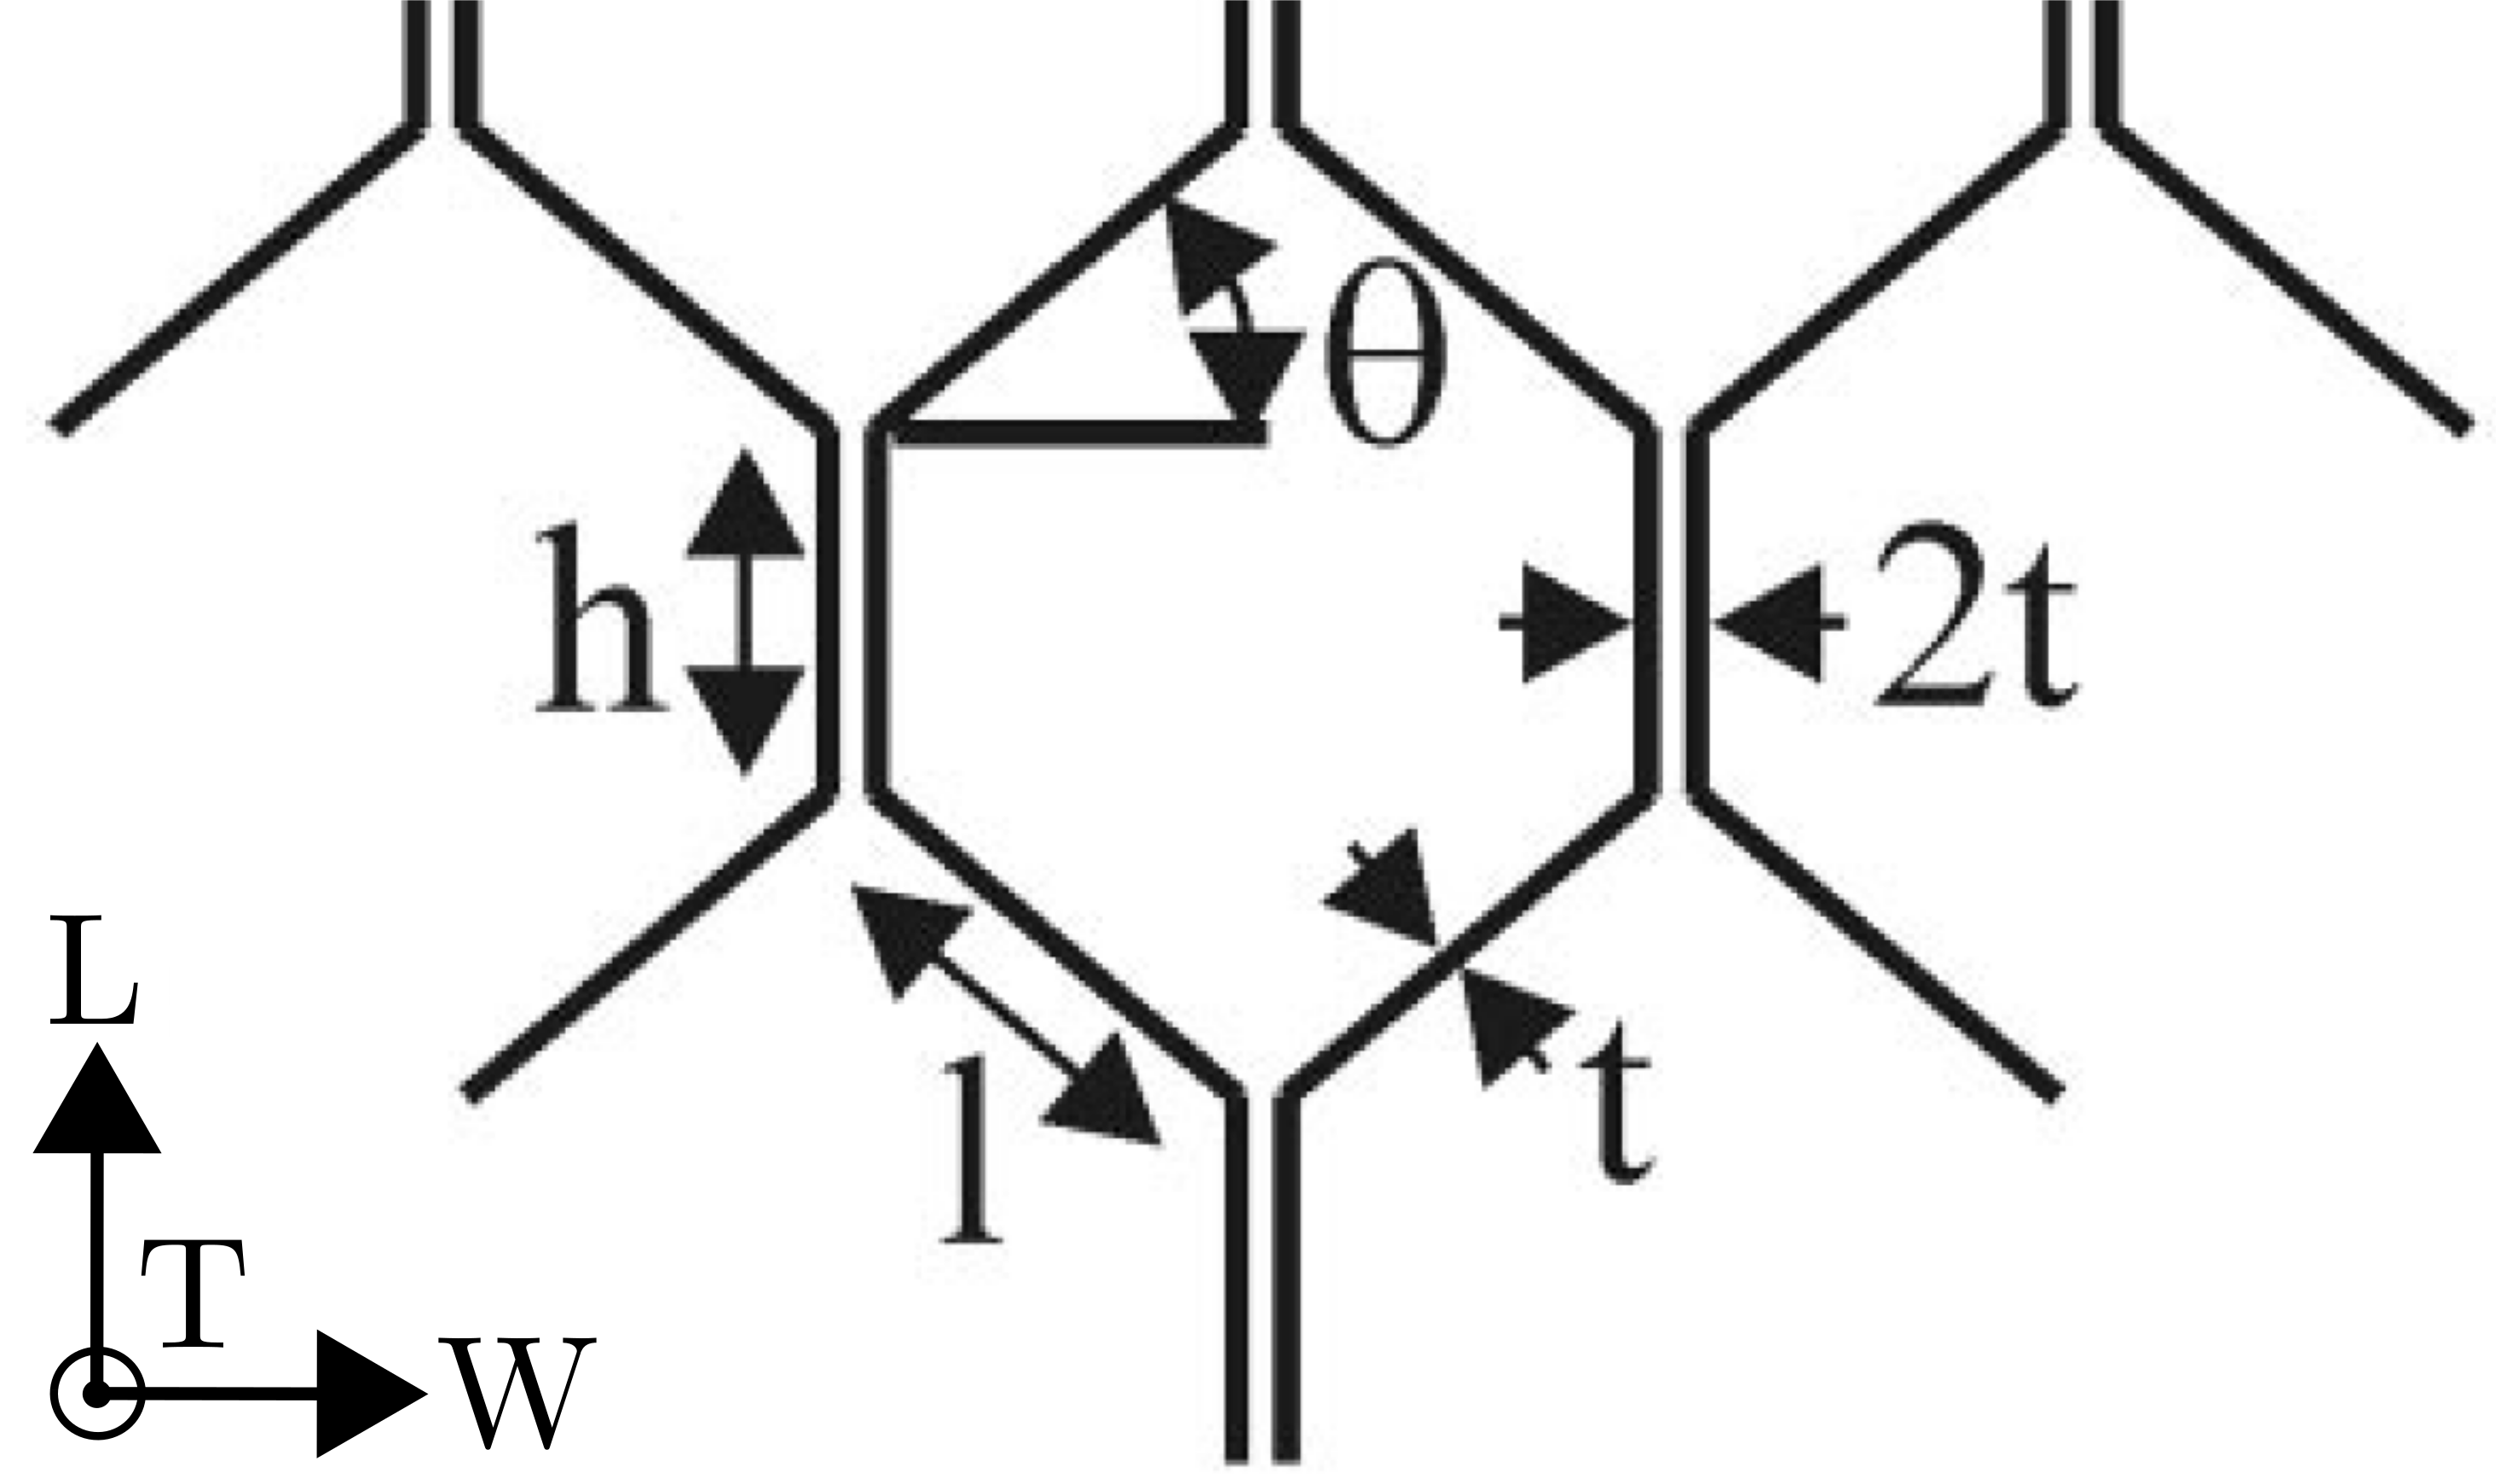
\includegraphics[width=0.4\linewidth]{./Images/Ch2/Ch2_topview_mod.PNG}
    \caption{Top-view of honeycomb structure. \cite{mohrdoyoyo2003}}
    \label{Ch2_topview}
\end{figure}
The TLW-coordinate system as indicated in the figure is commonly used in literature on honeycomb mechanics. The T-direction is referred to as the out-of-plane direction, and runs along the length of the hexagonal cells. In the T-direction the anisotropy is most obvious, but also between the L- and W- directions the structure differs. Therefore, the material is typically regarded as orthotropic.\\

As described in literature \cite{mohrdoyoyo2004a,niedermeyer,popp,DAP}, the behavior of the aluminium honeycomb in the deformable barrier is dominated by the out-of-plane direction due to the large differences in stiffness between the in-plane directions (WW, LL and LW and out-of plane directions (TT, TL and TW) caused by the geometry of the material. Therefore, the focus in modeling the behavior of the aluminum honeycomb material is on accurately describing the out-of-plane behavior. {\color{red}{||POSSIBLY CREATE APPENDIX with in-plane material characteristics?||}} Figure \ref{Ch2_stressstrain} illustrates the macroscopic out-of-plane crushing behavior of the honeycomb that is typically observed in pure compression.

\begin{figure}[H]
    \centering
    \begin{subfigure}[b]{0.50\textwidth}
    \centering
        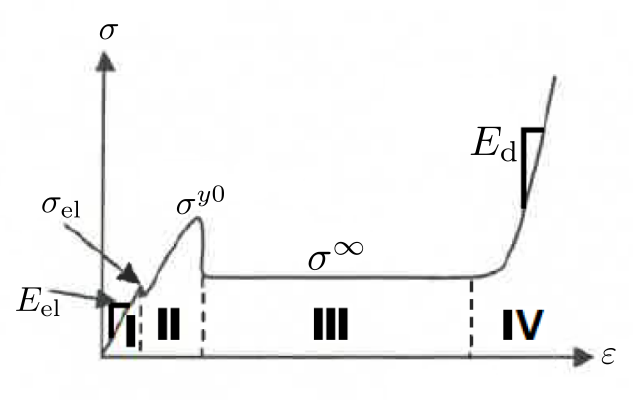
\includegraphics[width=1\textwidth]{./Images/Ch2/Ch2_stressstrain.PNG}
    \end{subfigure}
    \begin{subfigure}[b]{0.35\textwidth}
    \centering
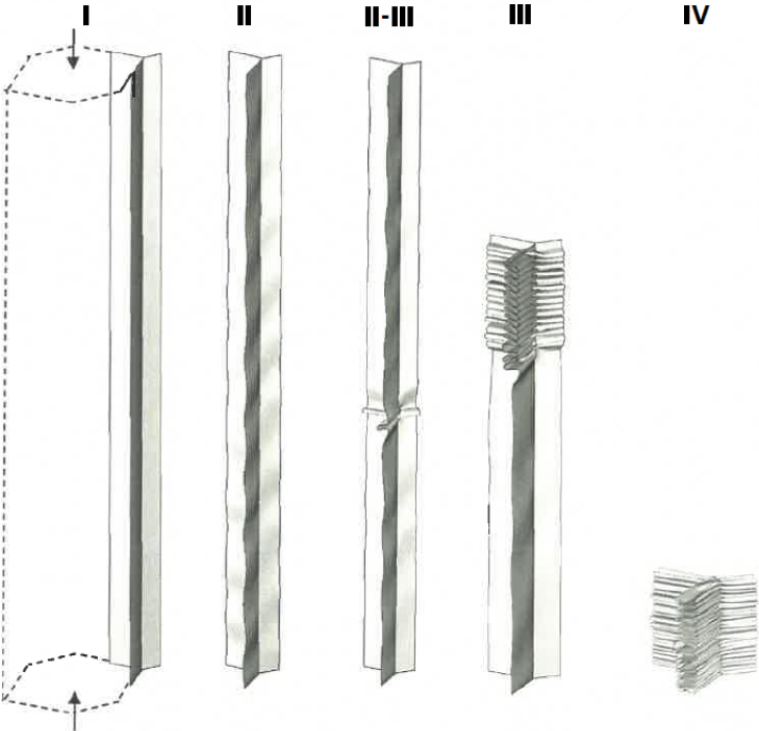
\includegraphics[width=1\textwidth]{./Images/Ch2/Ch2_crushfigure.PNG}
    \end{subfigure}
    \caption{Typical stress-strain response for compressive loading along the T-axis and the corresponding deformation behavior of a y-shaped unit cell.  \cite{niedermeyer}}
    \label{Ch2_stressstrain}
\end{figure}
\noindent In this response, the following four regimes are typically identified:
\begin{enumerate}[I]
    \item Linear elastic response.
    \item Nonlinear elastic response caused by the generation of elastic buckles in the micro-structure.
    \item Plastic buckling occurs and the stress level falls. Plastic folds appear in the micro-structure resulting in a long stress plateau. This strain softening leads to a localization front that travels through the material. 
    \item Densification occurs after crushing.
\end{enumerate}
Experiments show a strong coupling of out-of-plane compression loading with out-of-plane shear loading. This becomes particularly visible in the illustrations from Mohr \& Doyoyo \cite{mohrdoyoyo2004c} in Figure \ref{Ch2_shearbands}, where the folding patterns in the TW-plane are captured for pure compression (left) and compression under $\alpha = $60$^{\circ}$ (right) with respect to the W-axis. The folding direction indicated by the vector shows a dependency on the loading direction $\alpha$.
\begin{figure}[H]
    \centering
    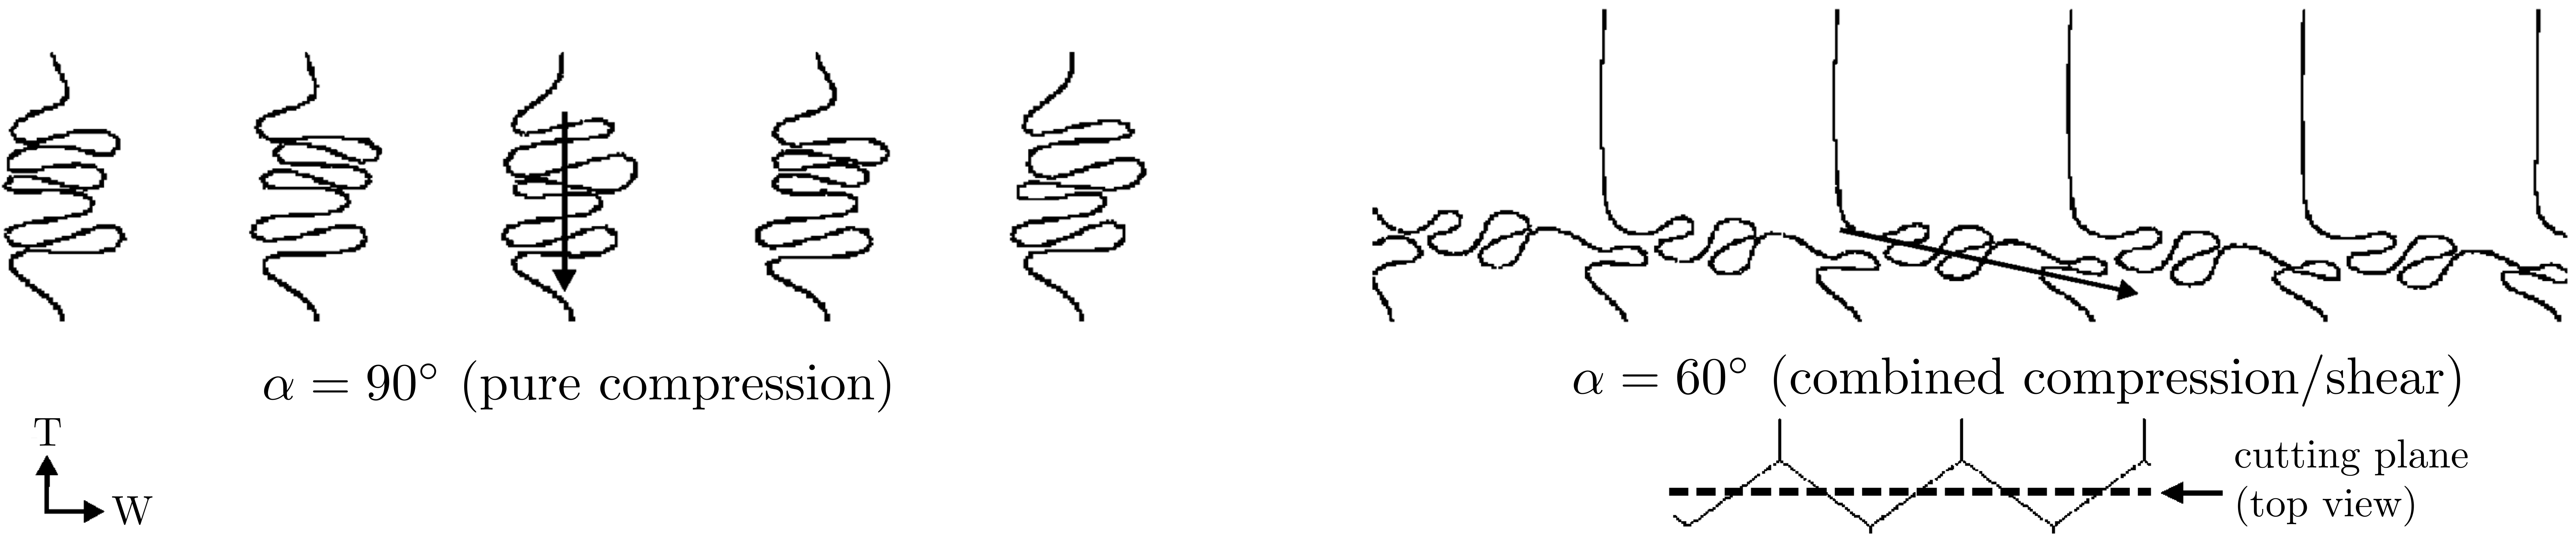
\includegraphics[width=\linewidth]{./Images/Ch2/Ch2_shearbands_cut2.PNG}
    \caption{Cuts through the folding micro-structure in the TW-plane for various loading angles with respect to the W-axis. The vector denotes the folding direction. \cite{mohrdoyoyo2004c}}
    \label{Ch2_shearbands}
\end{figure}
From these type of experiments, Mohr \& Doyoyo presented stress-strain curves in \cite{mohrdoyoyo2004b}. Figure \label{Ch2_MDexperiments} shows the curves for the normal direction (left) and for the shear direction (right). 
\begin{figure}[H]
    \centering
    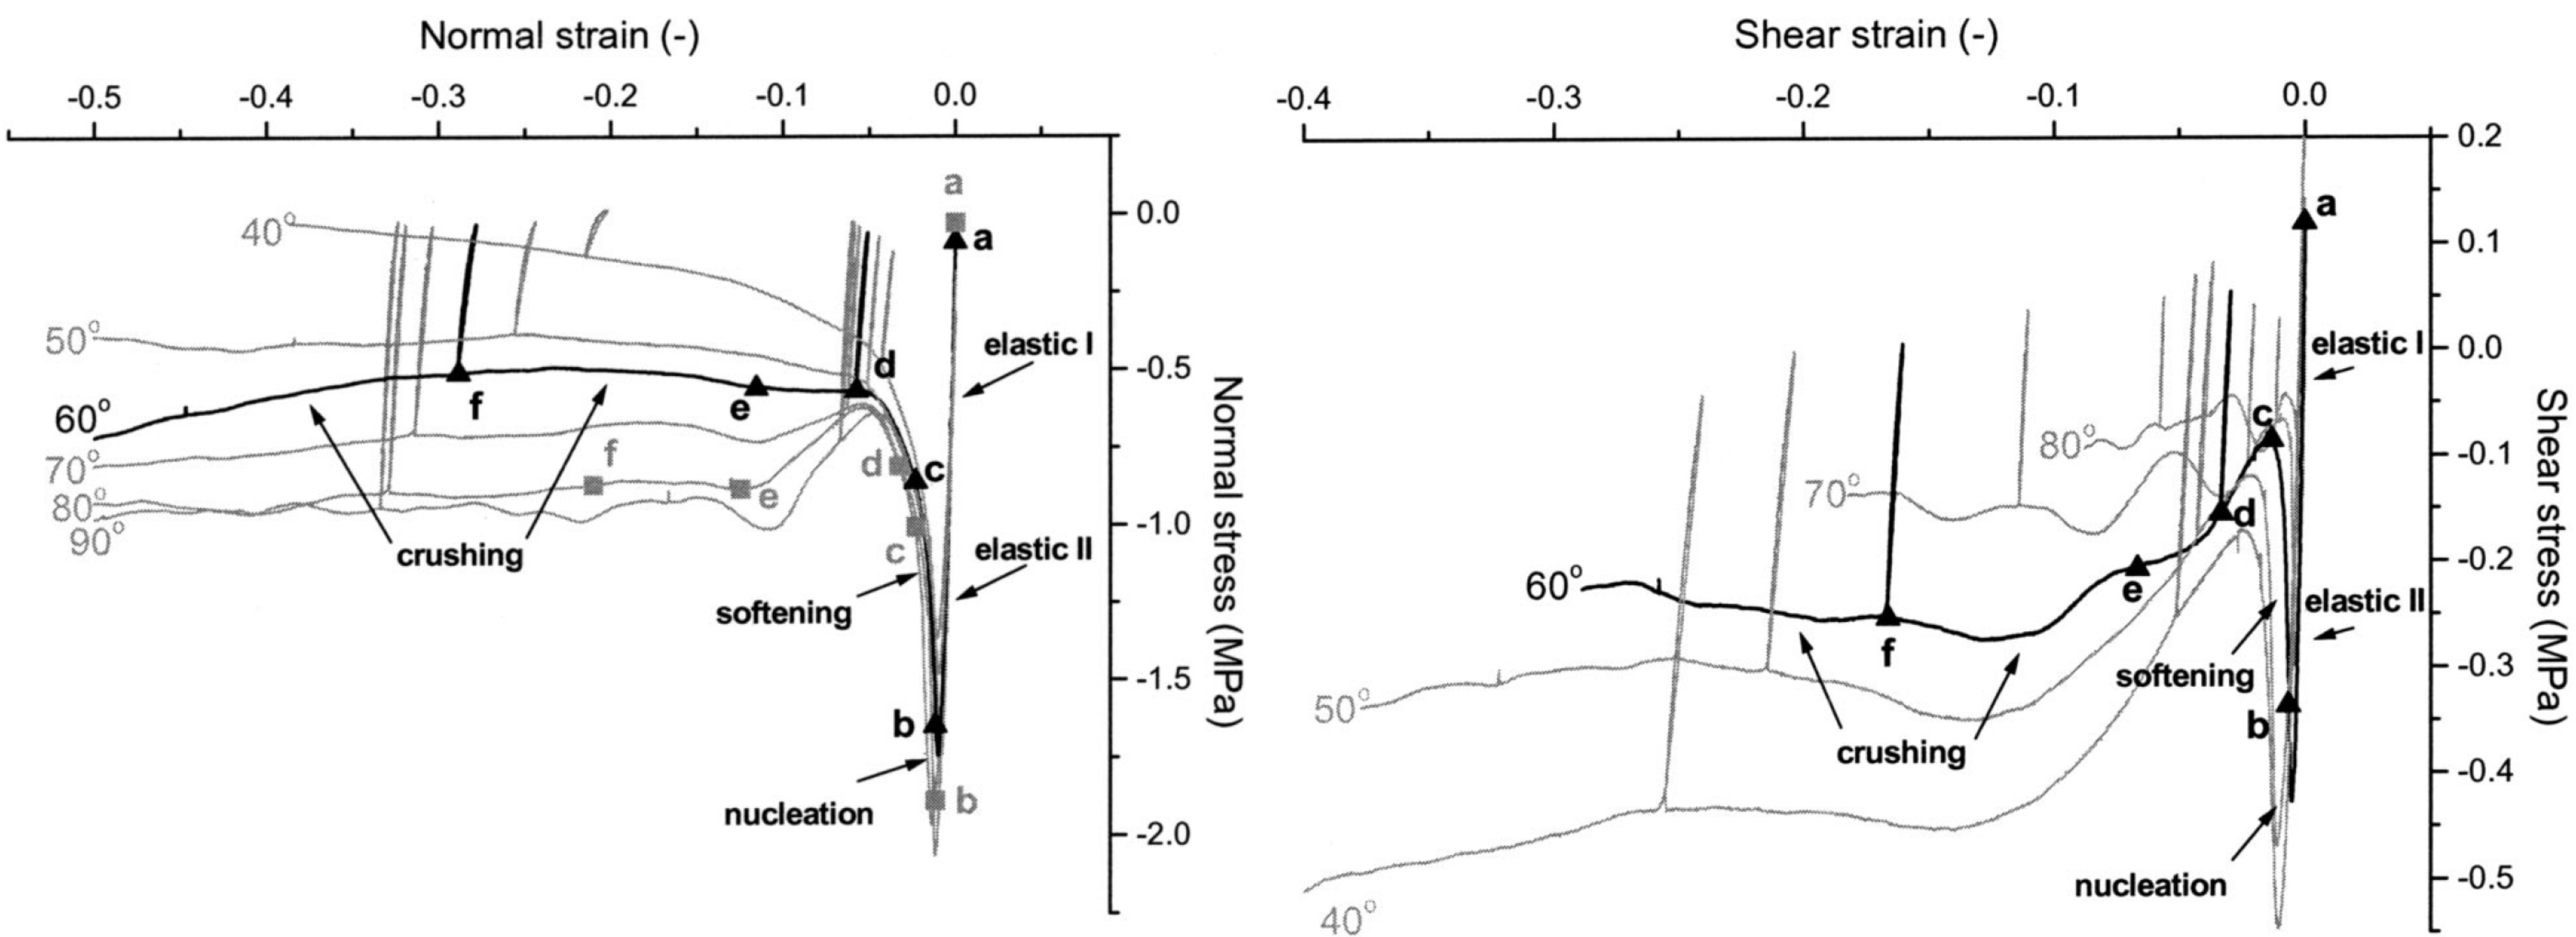
\includegraphics[width=\linewidth]{./Images/Ch2/Ch2_MDexperiments.png}
    \caption{Stress-strain curves for compression under an angle $\alpha$ with respect to the W-axis in the TW-plane in the normal direction (left) and in the shear direction (right). \cite{mohrdoyoyo2004b}}
    \label{Ch2_MDexperiments}
\end{figure}
Important to note here is that the crushing plateau remains relatively flat for all shown loading angles $\alpha$. Mohr \& Doyoyo used the stress-strain data to compose two typical failure envelopes which describe this out-of-plane shear and compression coupling. An example of these failure envelopes, corresponding to the stress-strain curves shown in the previous figure, are depicted in Figure \ref{Ch2_failenvelope}. The outer envelope describes the coupling for initial failure of the material, whereas the inner envelope describes the coupling during crushing.
\begin{figure}[H]
    \centering
    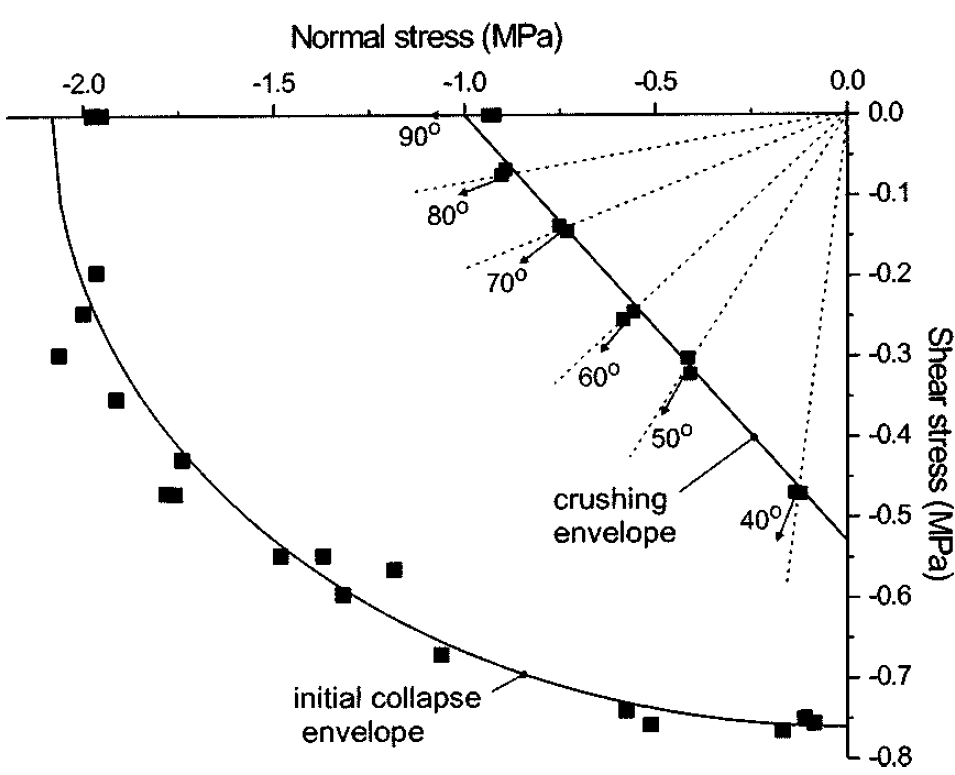
\includegraphics[width=0.55\linewidth]{./Images/Ch2/Ch2_failuremap.PNG}
    \caption{Failure envelopes for initial collapse and crushing under combined out-of-plane shear and compression loading. \cite{mohrdoyoyo2004b}}
    \label{Ch2_failenvelope}
\end{figure}
These failure envelopes are captured by Equations \ref{Ch2_eq_failenv1} and \ref{Ch2_eq_failenv2}, \cite{mohrdoyoyo2004b}. Here $\sigma_{TT}^{y0}$ and $\sigma_{TT}^{\infty}$ denote the initial yield stress and the crushing stress for compression along the T-axis respectively. $\tau_{TW}^{y0}$ and $\tau_{TW}^{\infty}$ denote the initial yield stress and the crushing stress for shear in the TW plane respectively. 
\begin{subequations}
\begin{equation}
    \Big(\frac{\sigma_{TT}}{\sigma^{y0}_{TT}}\Big)^2+\Big(\frac{\tau_{TW}}{\tau^{y0}_{TW}}\Big)^2 = 1 \quad \text{(initial collapse)},
    \label{Ch2_eq_failenv1}
\end{equation}
\begin{equation}
    \frac{\sigma_{TT}}{\sigma^{\infty}_{TT}} + \left| \frac{\tau_{TW}}{\tau^{\infty}_{TW}}\right| = 1  \quad \text{(crushing)}.
    \label{Ch2_eq_failenv2}
\end{equation}
\label{Ch2_eq_failenv}
\end{subequations}
{\color{red}{Bruggetje naar volgende hoofdstuk}}
\subsection{Modeling techniques}
Capturing the described mechanics in a numerical model has been subject of significant research efforts. These research efforts can be roughly divided into two categories: shell models and continuum models. 
\subsubsection{Shell models}
Shell models are the current industry standard. In shell models, the hexagonal cell structure is incorporated in the models. Therefore, this type of models inherently capture the geometric effects of the material. Figure \ref{Ch2_weerts} from Weerts \cite{weerts} shows a typical way of simplifying the buckling behavior of honeycomb structures under compression. In stead of modeling the folding pattern in detail, so called 'crushing elements' are used.
\begin{figure}[H]
    \centering
    \begin{subfigure}[b]{0.48\linewidth}
        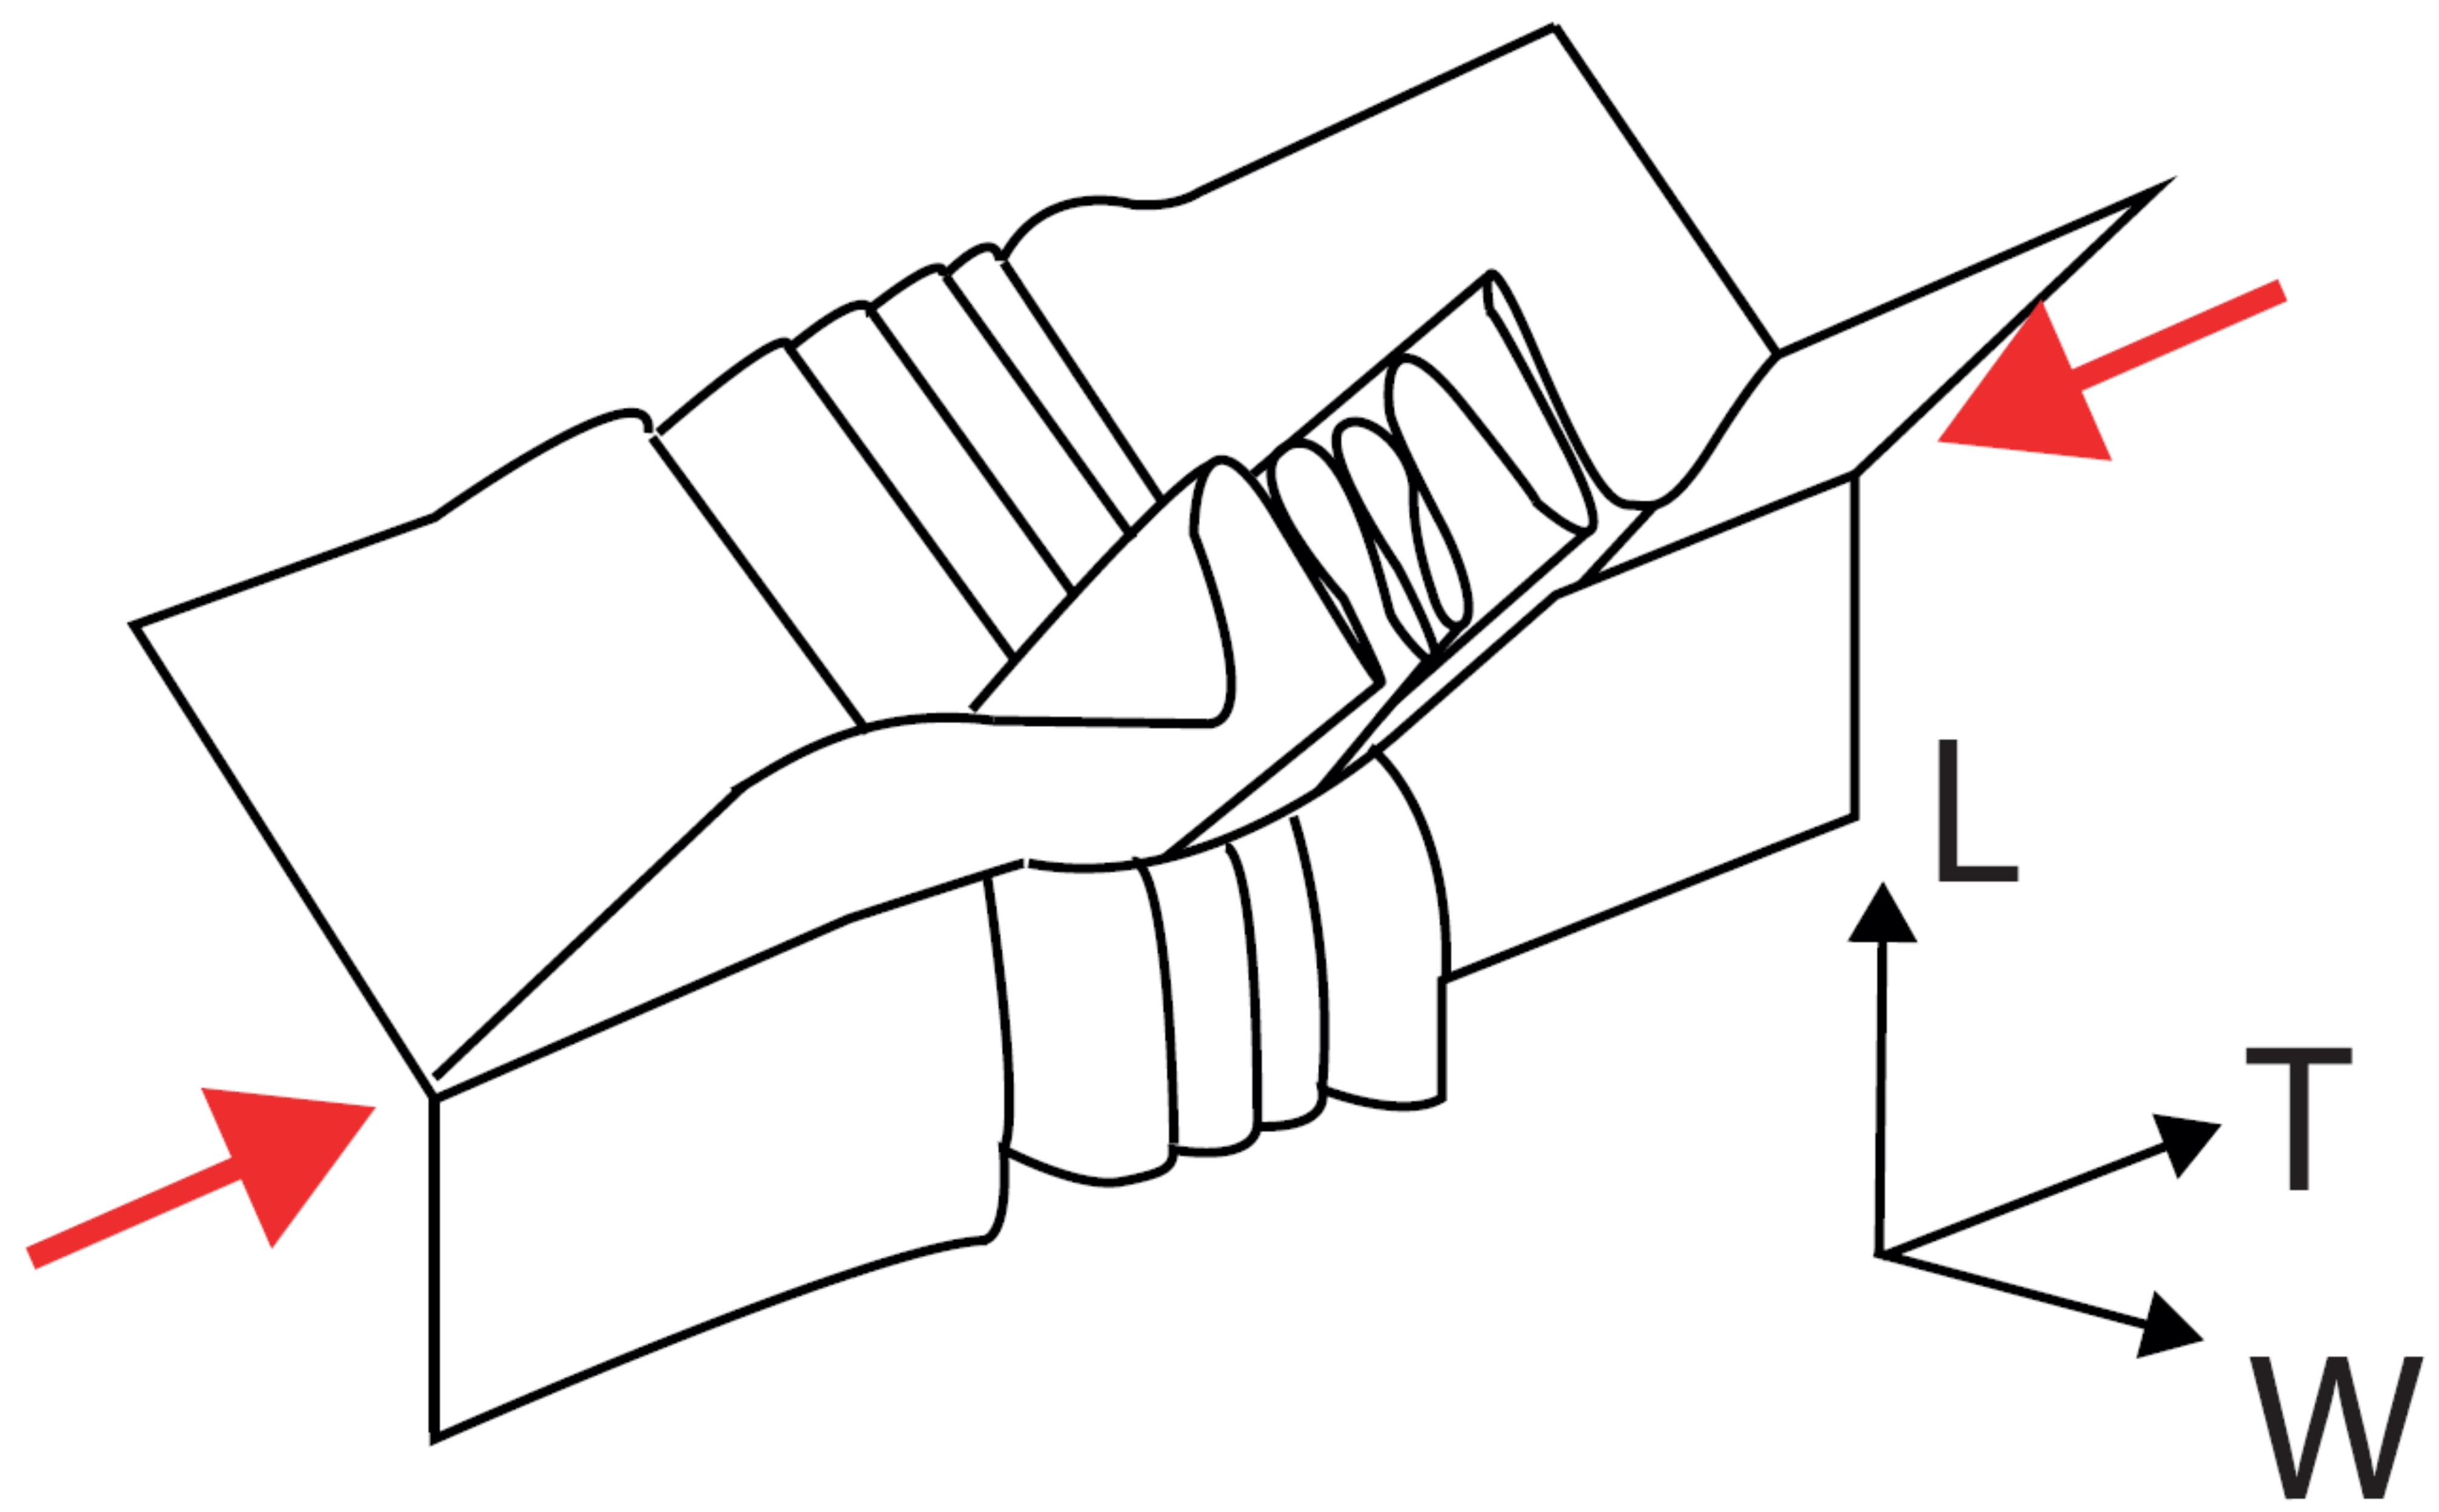
\includegraphics[width=0.7\linewidth]{./Images/Ch2/Ch2_weerts_detailed.png}
        \caption{Detailed model: Buckling of cell walls.}
        \label{Ch2_weerts_detailed}
    \end{subfigure}
    %add desired spacing between images, e. g. ~, \quad, \qquad, \hfill etc. %(or a blank line to force the subfigure onto a new line)
    \begin{subfigure}[b]{0.48\linewidth}
        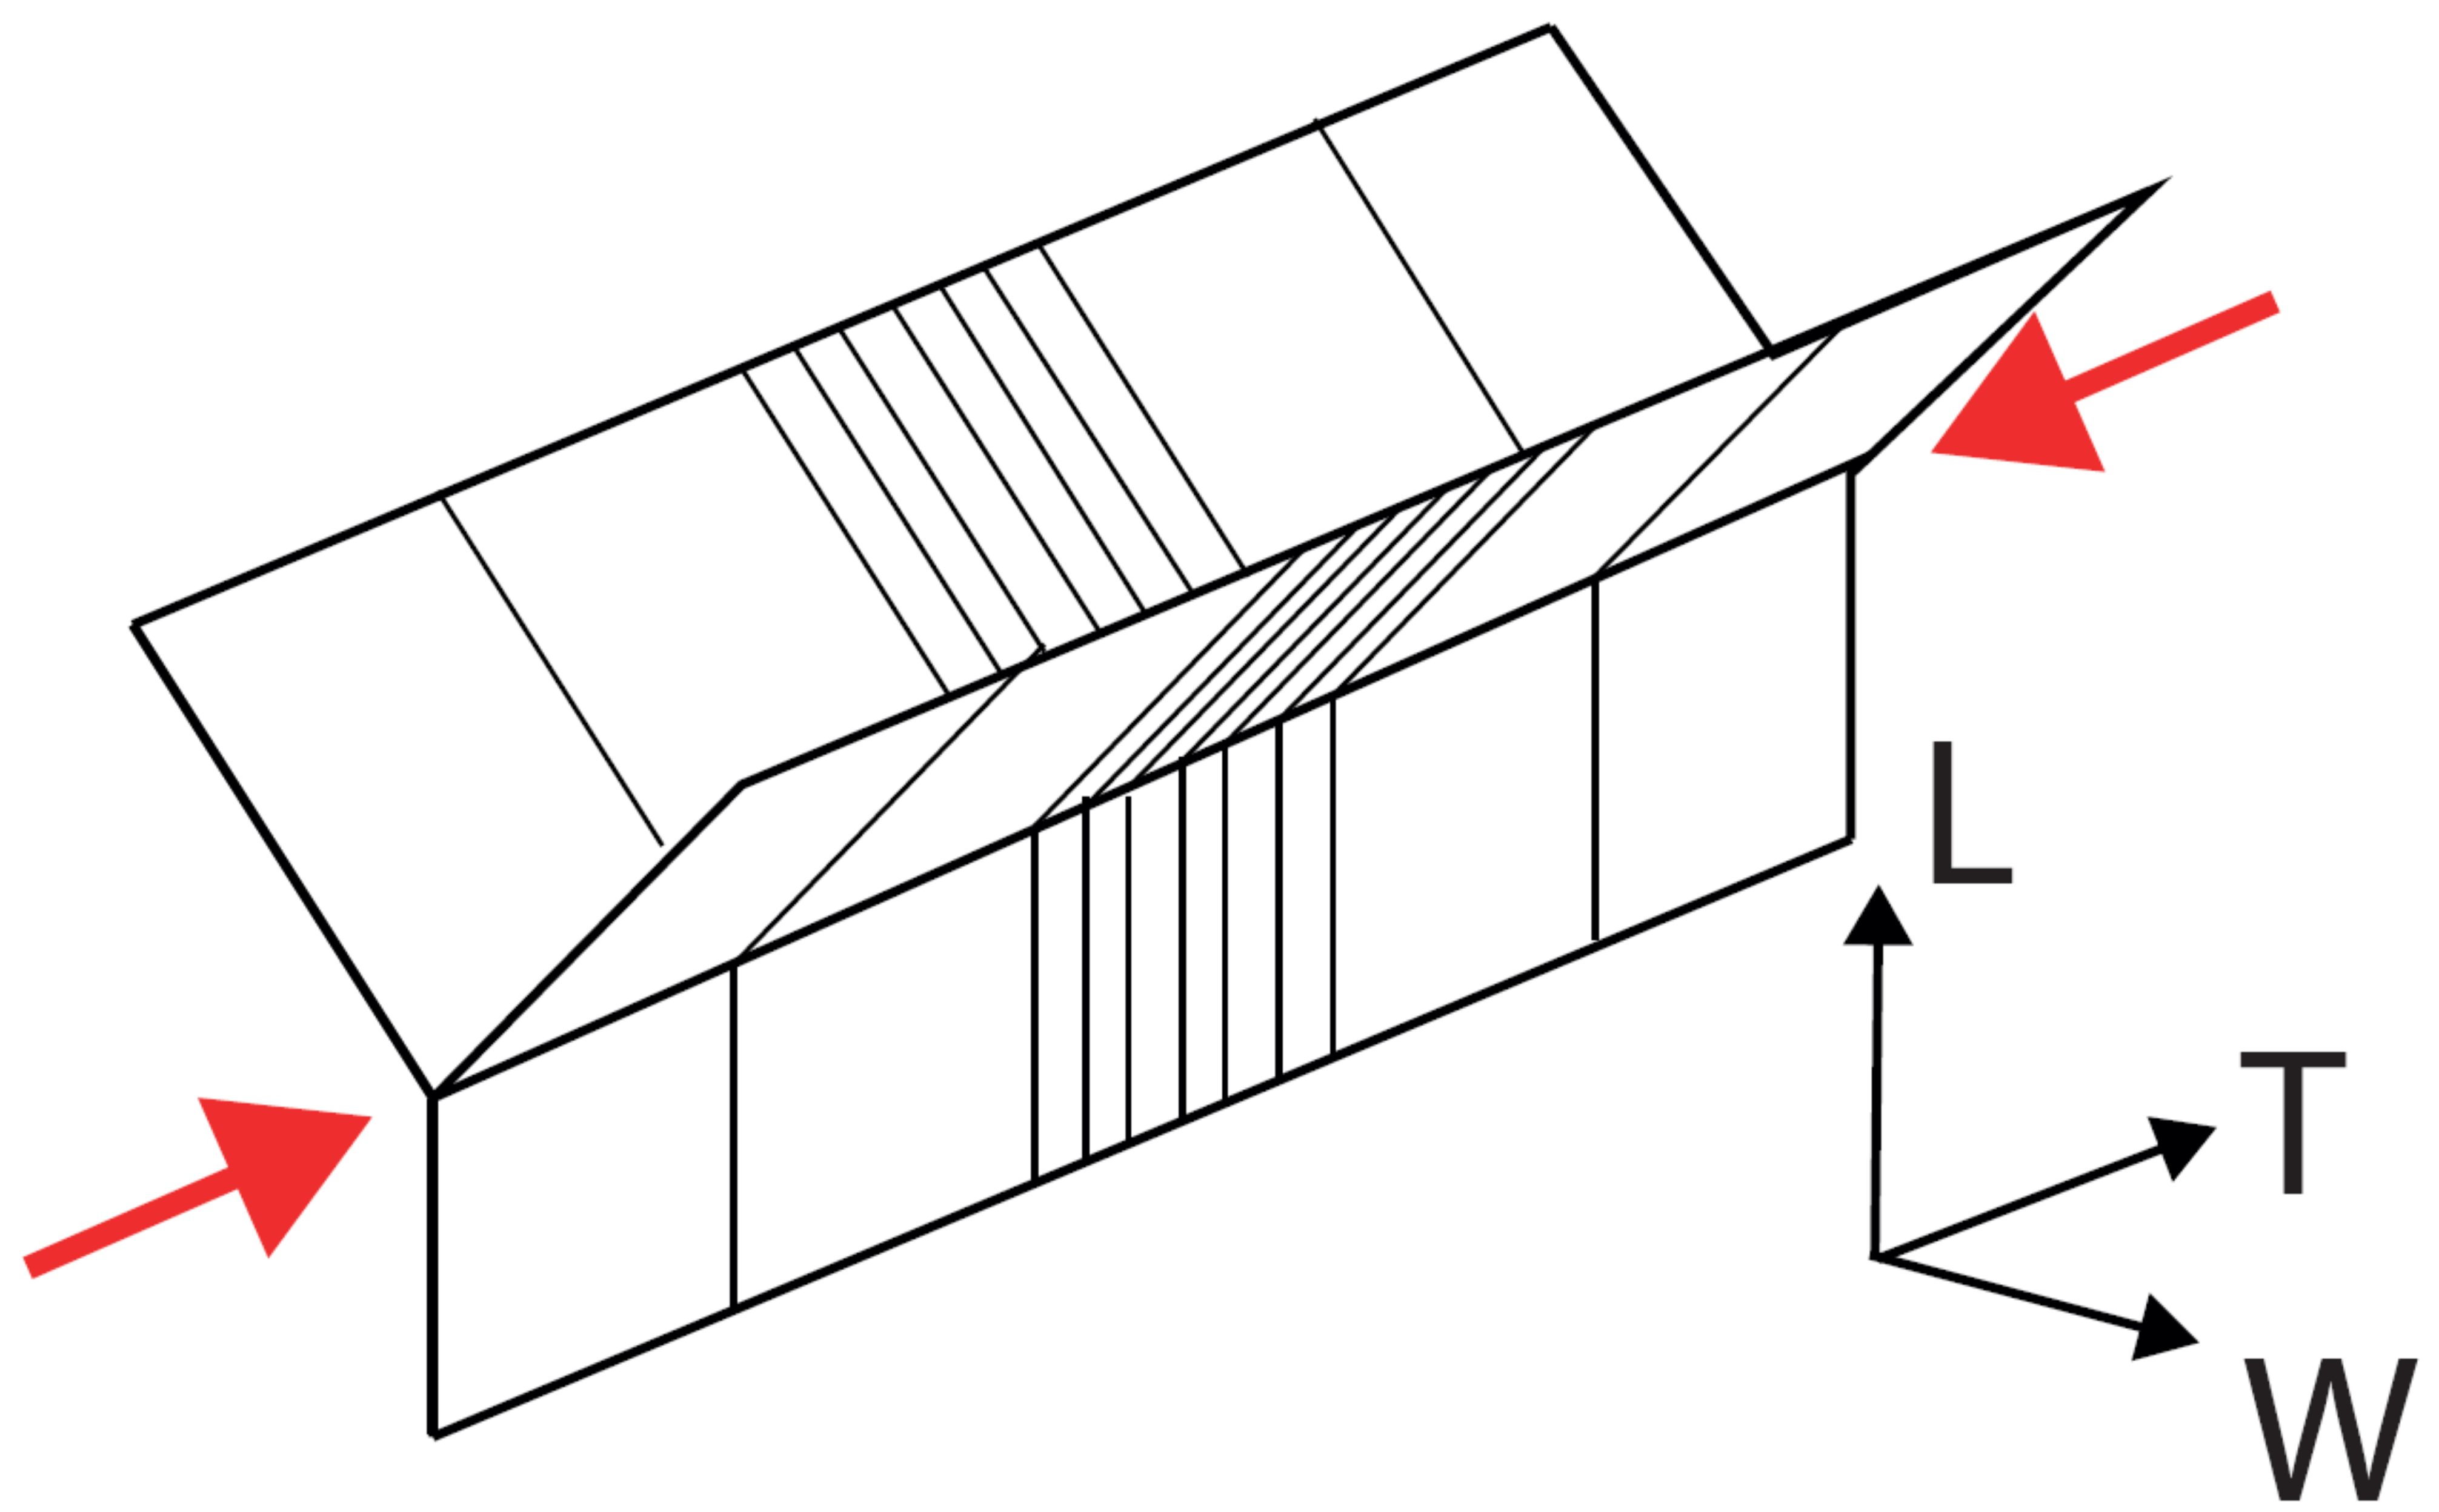
\includegraphics[width=0.7\linewidth]{./Images/Ch2/Ch2_weerts_coarse.png}
         \caption{Coarse model: Crushing of elements.}
          \label{Ch2_weerts_coarse}
    \end{subfigure}
    \caption{Two shell modeling approaches. \cite{weerts}}
    \label{Ch2_weerts}
\end{figure}
Niedermeyer \cite{niedermeyer} showed that 24 elements are needed per honeycomb wall to model the out-of-plane buckling with an error of less than 10\%. This is the primary reason why the current BMW shell models use the geometrically simplified crushing elements shown in Figure \ref{Ch2_weerts_coarse}. Weerts \cite{weerts} performed an optimization of the in-plane properties of these shell models with crushing elements to obtain accurate results. Due to the progressive crushing of consecutive elements, a localization front appears which resembles the observations from experiments.{\color{red}{NADEEL VAN SHELL MODELS NOEMEN -> dap noemt mesh dependency}}\\

\subsubsection{Continuum models}
In continuum models, the mechanical behavior of the honeycomb structure is homogenized. The hexagonal cell structure does not have to be incorporated in the model, resulting in a model of which the geometry is more simple. However, since the geometric effects caused by the cell structure are not inherently captured in the model, these must be accounted for by the material model. Potentially there is an efficiency gain in modeling the honeycomb block with continuum elements, if the material model does not become overly complex.\\
Popp \cite{popp} described a homogenized model which includes the coupling between out-of-plane compression and out-of-plane shear based on formulations proposed by Mohr \& Doyoyo \cite{mohrdoyoyo2004a}. Promising results were obtained regarding the averaged force response of the honeycomb material. Figure \ref{Ch2_poppdap} shows an illustration of the stress-strain response as observed in experiments (left) and the response based on the model of Popp (right) under pure compression.  Due to the absence of the strain-softening after initial buckling in the model of Popp, the localization front which is observed during experiments is not captured. In stead, the blocks deformation is nearly homogeneous.
\begin{figure}[H]
    \centering
    \begin{subfigure}[b]{0.48\linewidth}
        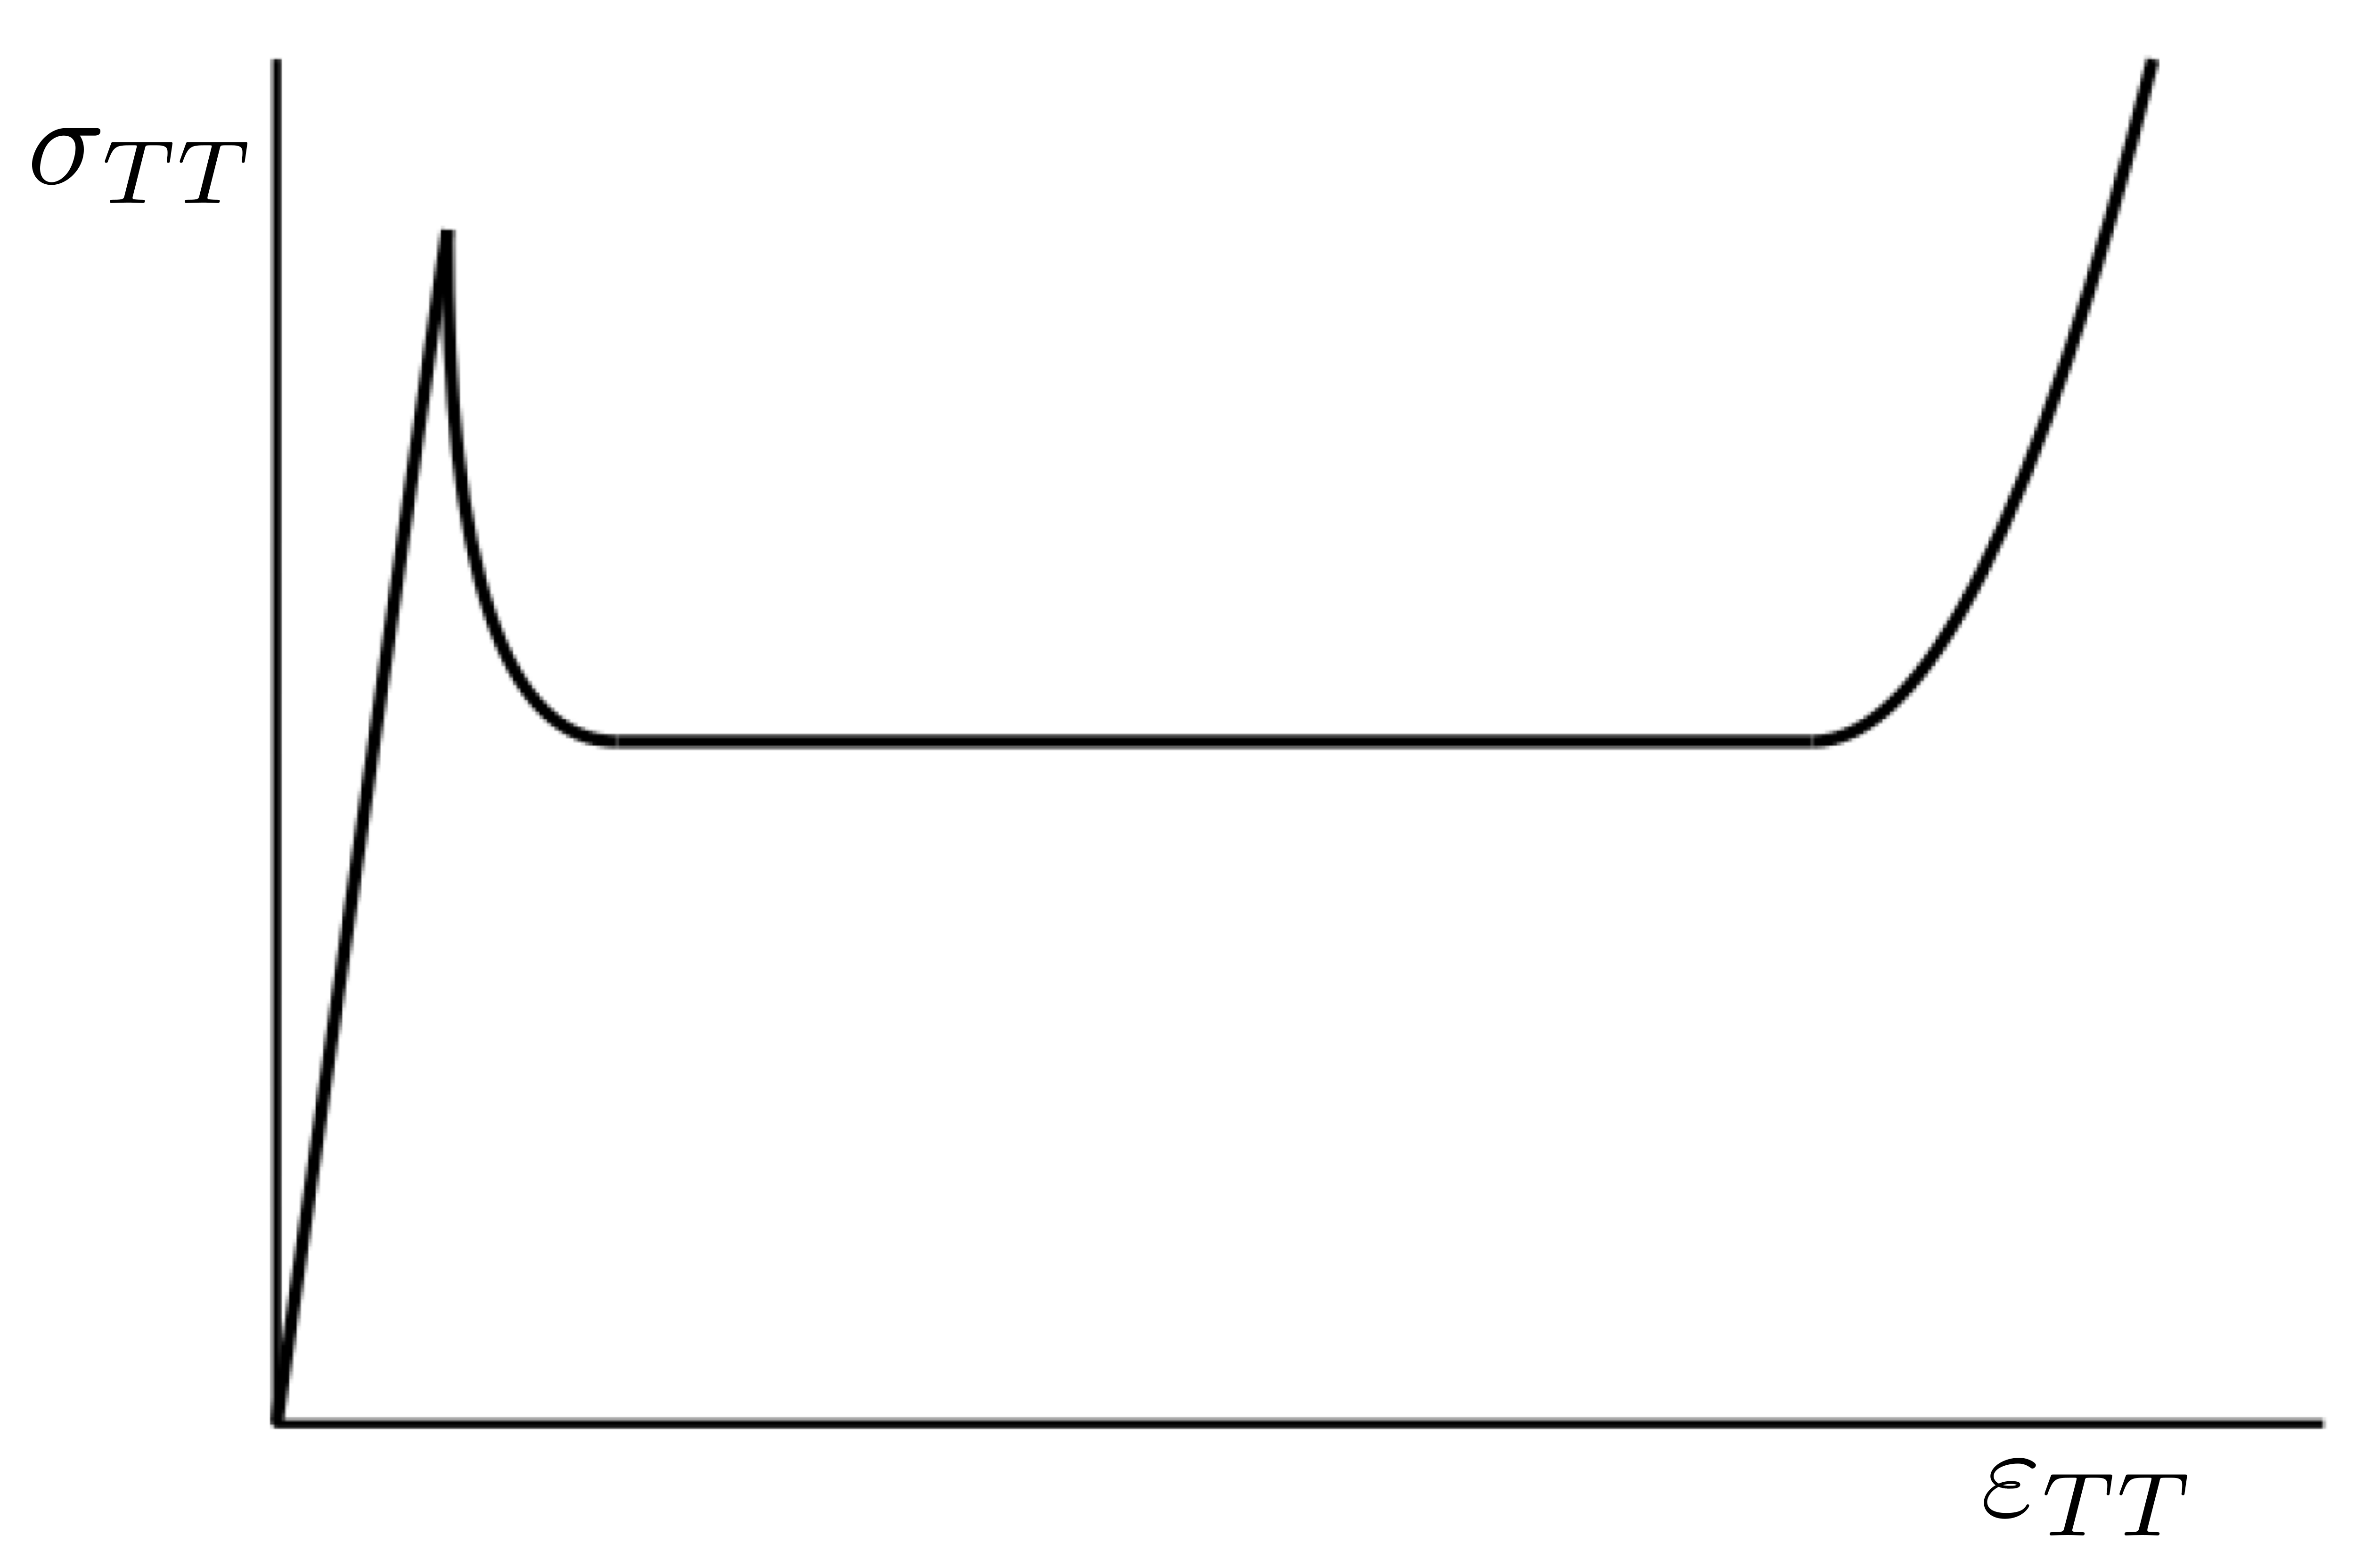
\includegraphics[width=0.7\linewidth]{./Images/Ch2/Ch2_dap_popp_dap.png}
        \caption{}
        \label{Ch2_poppdap1}
    \end{subfigure}
    %add desired spacing between images, e. g. ~, \quad, \qquad, \hfill etc. %(or a blank line to force the subfigure onto a new line)
    \begin{subfigure}[b]{0.48\linewidth}
        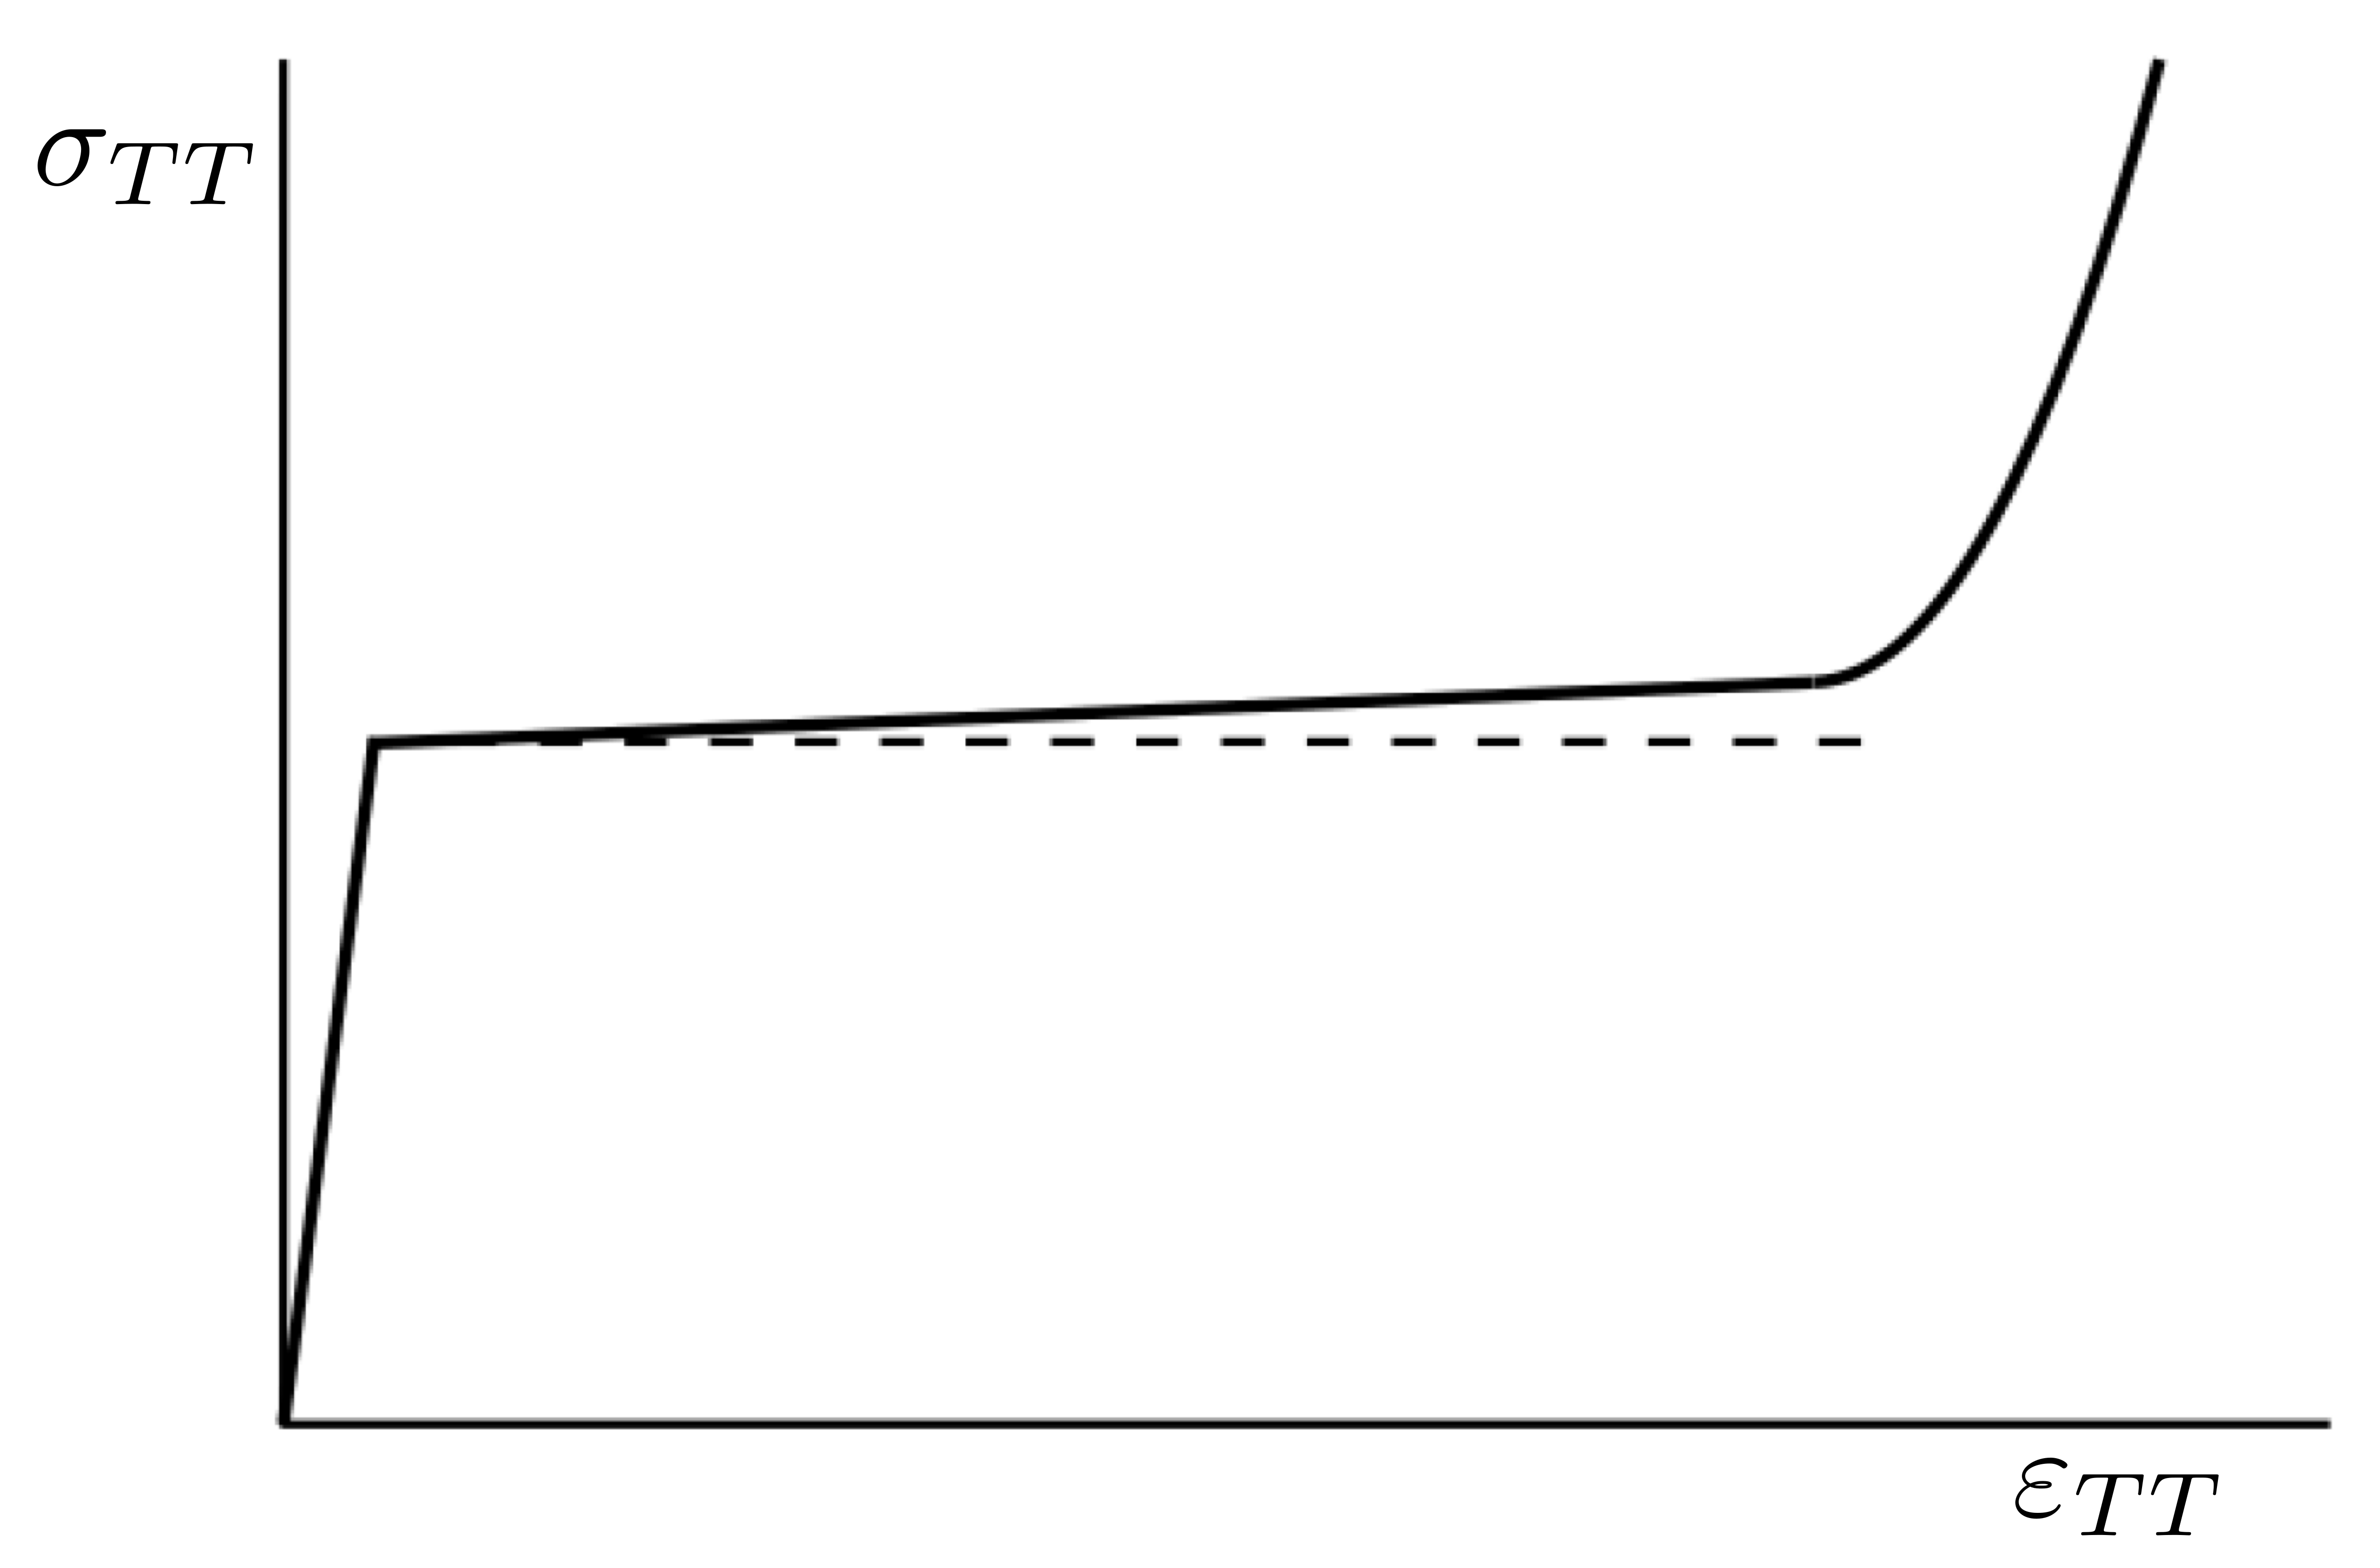
\includegraphics[width=0.7\linewidth]{./Images/Ch2/Ch2_dap_popp_popp.png}
         \caption{}
          \label{Ch2_poppdap2}
    \end{subfigure}
    \caption{Stress-strain curve of a aluminium honycomb (a) in reality versus (b) the material model implemented by Popp.\cite{DAP}}
    \label{Ch2_poppdap}
\end{figure}
Van Iersel \cite{DAP} also focused on models based on continuum elements. In that work, a phenomenological model was created that did capture the strain-softening after initial buckling. Van Iersel adopted a non-local formulation to limit the mesh dependency that arises due to the strain-softening. This resulted in a promising three dimensional model in which the localization front is captured, and a force response which is in accordance with experimental data for pure compression. Figure \ref{Ch2_dap_deformedblock} shows the localization front traveling through the material, as each row of elements subsequently collapses.
\begin{figure}[H]
    \centering
    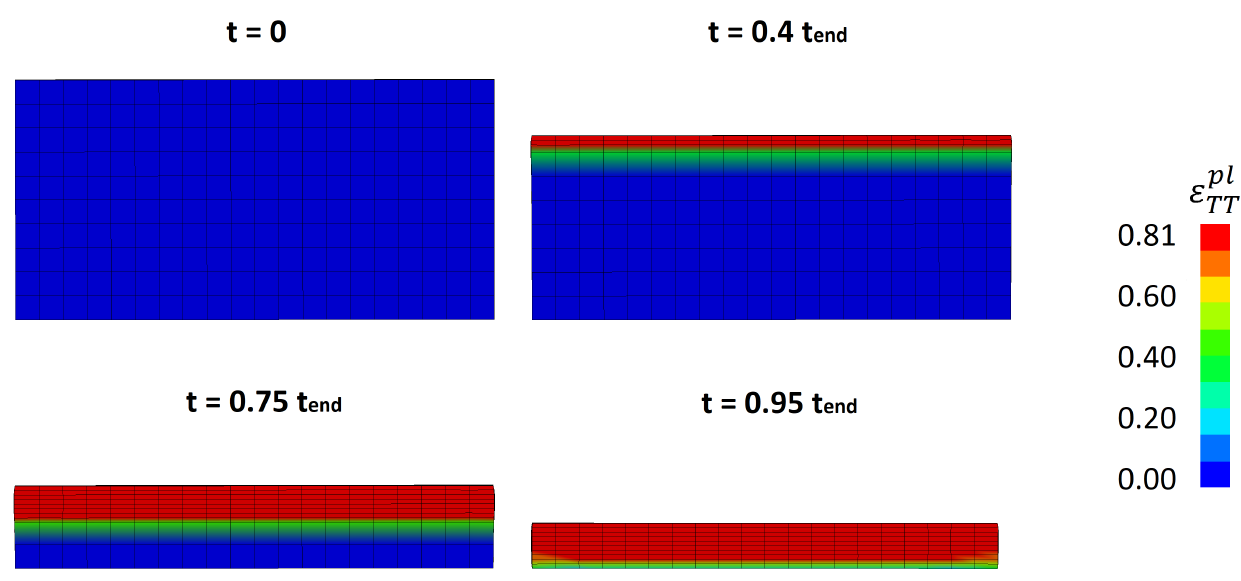
\includegraphics[width=0.75\linewidth]{./Images/Ch2/Ch2_dap_deformedblock.PNG}
    \caption{Local plastic strain and deformed mesh for 4 points in time, a mesh with 10 elements along the T-axis. \cite{DAP}}
    \label{Ch2_dap_deformedblock}
\end{figure}
However, during simulations with a combined shear and compression loading, non-physical behavior was observed for large shear strains. Still, the results of the homogenised non-local continuum element formulation of Van Iersel show the potential of continuum models to be more computationally efficient than the shell models currently used in industry. In this thesis, the continuum model of Van Iersel will be modified for the use of large (shear) deformations. Section \ref{Ch2_sec_improvements} will be dedicated to pinpointing the cause of the non-physical behavior of the model proposed by Van Iersel under high shear loading. 

\subsection{Inconsistencies in continuum model}
The non-phyiscal behavior in the model of Van Iersel is most clearly observed in the stress-strain response in the normal direction of a single element which is compressed under an angle $\alpha$ in Figure \ref{Ch2_dap_shearstress}.
\begin{figure}[H]
    \centering
    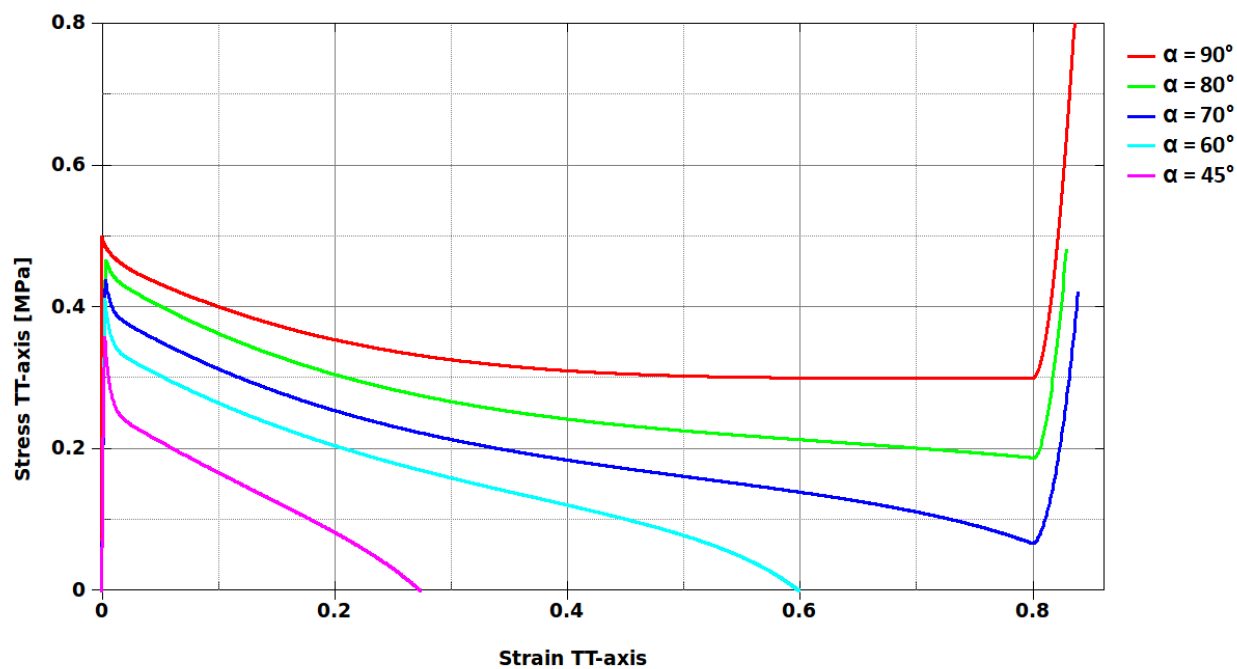
\includegraphics[width=0.9\linewidth]{./Images/Ch2/Ch2_dap_shearstress.PNG}
    \caption{Stress-strain response along TT-axis of a single element for varying loading angles.\cite{DAP}}
    \label{Ch2_dap_shearstress}
\end{figure}
For pure compression loading ($\alpha = 90^{\circ}$) the stress-strain response corresponds to the typical behavior of a honeycomb as was described in Section 2.1. However, when the shear component is increased by decreasing the loading angle $\alpha$, the stress-strain behavior starts to deviate from what is expected based on the experimentally observed behavior of Figure \ref{Ch2_MDexperiments}. There, a relatively straight crushing plateau was observed for loading angles between $90^{\circ}$ and $50^{\circ}$.\\
\newline
The non-physical behavior in the model of Van Iersel is caused by the kinematics of the implemented strain definition. Van Iersel uses the Biot strain tensor based on the right stretch tensor $\boldsymbol{U}$. The Biot strain is defined as:
\begin{equation}
    \boldsymbol{\varepsilon}_{\text{Biot}} = \boldsymbol{U} - \boldsymbol{I},
\end{equation}
with $\boldsymbol{I}$ the second order unit tensor. With the right polar decomposition, the deformation gradient tensor $\boldsymbol{F}$ is decomposed into a symmetric stretch tensor $\boldsymbol{U}$ and a rotation tensor $\boldsymbol{R}$. In figure \ref{Ch2_right_polar_decomp} from \cite{DAP}, a shear deformation is sketched in 2D. The figure illustrates that, during this type of deformation, a rotation is introduced in order to keep the stretch tensor $\boldsymbol{U}$ symmetric. Due to this rotation, a misalignment arises between the orthogonal basis in which the material model is defined and the orthogonal basis in which the strains are computed. The rotation angle that is needed to keep $\boldsymbol{U}$ symmetric increases for larger shear strains. This explains why the predictions of the model of Van Iersel deviate more for lower loading angles $\alpha$. Only during pure compression ($\alpha = 90^{\circ}$ this model as currently implemented will yield sensible results, since in that case the right polar decomposition of the deformation gradient tensor will result in a rotation tensor of $\boldsymbol{R}=\boldsymbol{I}$.
\begin{figure}[H]
    \centering
    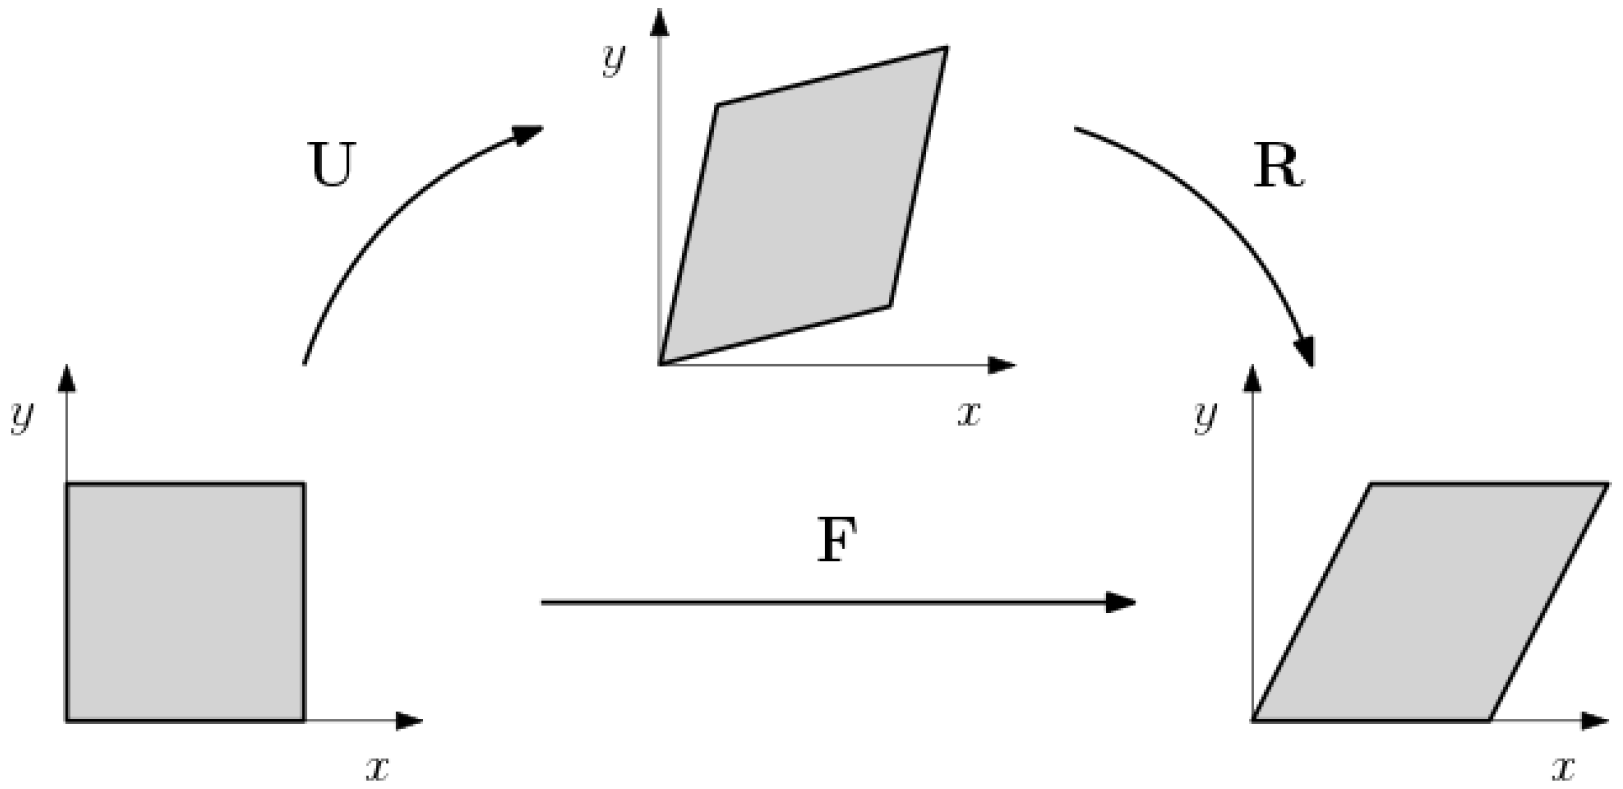
\includegraphics[width=0.9\linewidth]{./Images/Ch2/Ch2_right_polar_decomp.PNG}
    \caption{Schematic representation of the kinematic behavior for shear deformation.\cite{DAP}}
    \label{Ch2_right_polar_decomp}
\end{figure}
In the next section, a finite deformation model based on the implementations of Van Iersel will be described in order to eliminate this undesired behavior of the model . 

\label{Ch2_sec_improvements}